
\documentclass[letterpaper,hide notes,xcolor={table,svgnames},pdftex,10pt]{beamer}
\def\showexamples{t}


%\usepackage[svgnames]{xcolor}

%% Demo talk
%\documentclass[letterpaper,notes=show]{beamer}

\usecolortheme{crane}
\setbeamertemplate{navigation symbols}{}

\usetheme{MyPittsburgh}
%\usetheme{Frankfurt}

%\usepackage{tipa}

\usepackage{hyperref}
\usepackage{graphicx,xspace}
\usepackage[normalem]{ulem}
\usepackage{multicol}
\usepackage{amsmath,amssymb,amsthm,graphicx,xspace}
\newcommand\SF[1]{$\bigstar$\footnote{SF: #1}}

\usepackage[default]{sourcesanspro}
\usepackage[T1]{fontenc}
\usepackage[scaled]{beramono}
\usepackage{tikzpagenodes}

\newcounter{tmpnumSlide}
\newcounter{tmpnumNote}


% old question code
%\newcommand\question[1]{{$\bigstar$ \small \onlySlide{2}{#1}}}
% \newcommand\nquestion[1]{\ifdefined \presentationonly \textcircled{?} \fi \note{\par{\Large \textbf{?}} #1}}
% \newcommand\nanswer[1]{\note{\par{\Large \textbf{A}} #1}}


 \newcommand\mnote[1]{%
   \addtocounter{tmpnumSlide}{1}
   \ifdefined\showcues {~\tiny\fbox{\arabic{tmpnumSlide}}}\fi
   \note{\setlength{\parskip}{1ex}\addtocounter{tmpnumNote}{1}\textbf{\Large \arabic{tmpnumNote}:} {#1\par}}}

\newcommand\mmnote[1]{\note{\setlength{\parskip}{1ex}#1\par}}

%\newcommand\mnote[2][]{\ifdefined\handoutwithnotes {~\tiny\fbox{#1}}\fi
% \note{\setlength{\parskip}{1ex}\textbf{\Large #1:} #2\par}}

%\newcommand\mnote[2][]{{\tiny\fbox{#1}} \note{\setlength{\parskip}{1ex}\textbf{\Large #1:} #2\par}}

\newcommand\mquestion[2]{{~\color{red}\fbox{?}}\note{\setlength{\parskip}{1ex}\par{\Large \textbf{?}} #1} \note{\setlength{\parskip}{1ex}\par{\Large \textbf{A}} #2\par}\ifdefined \presentationonly \pause \fi}

\newcommand\blackboard[1]{%
\ifdefined   \showblackboard
  {#1}
  \else {\begin{center} \fbox{\colorbox{blue!30}{%
         \begin{minipage}{.95\linewidth}%
           \hspace{\stretch{1}} Some space intentionally left blank; done at the blackboard.%
         \end{minipage}}}\end{center}}%
         \fi%
}



%\newcommand\q{\tikz \node[thick,color=black,shape=circle]{?};}
%\newcommand\q{\ifdefined \presentationonly \textcircled{?} \fi}

\usepackage{listings}
\lstset{basicstyle=\footnotesize\ttfamily,
	breaklines=true,
	aboveskip=15pt,
  	belowskip=15pt,
	frame=lines,
	numbers=left, basicstyle=\scriptsize, numberstyle=\tiny, stepnumber=0, numbersep=2pt
}

\usepackage{siunitx}
\newcommand\sius[1]{\num[group-separator = {,}]{#1}\si{\micro\second}}
\newcommand\sims[1]{\num[group-separator = {,}]{#1}\si{\milli\second}}
\newcommand\sins[1]{\num[group-separator = {,}]{#1}\si{\nano\second}}
\sisetup{group-separator = {,}, group-digits = true}

%% -------------------- tikz --------------------
\usepackage{tikz}
\usetikzlibrary{positioning}
\usetikzlibrary{arrows,backgrounds,automata,decorations.shapes,decorations.pathmorphing,decorations.markings,decorations.text,decorations.pathreplacing}

\tikzstyle{place}=[circle,draw=blue!50,fill=blue!20,thick, inner sep=0pt,minimum size=6mm]
\tikzstyle{transition}=[rectangle,draw=black!50,fill=black!20,thick, inner sep=0pt,minimum size=4mm]

\tikzstyle{block}=[rectangle,draw=black, thick, inner sep=5pt]
\tikzstyle{bullet}=[circle,draw=black, fill=black, thin, inner sep=2pt]

\tikzstyle{pre}=[<-,shorten <=1pt,>=stealth',semithick]
\tikzstyle{post}=[->,shorten >=1pt,>=stealth',semithick]
\tikzstyle{bi}=[<->,shorten >=1pt,shorten <=1pt, >=stealth',semithick]

\tikzstyle{mut}=[-,>=stealth',semithick]

\tikzstyle{treereset}=[dashed,->, shorten >=1pt,>=stealth',thin]

\usepackage{ifmtarg}
\usepackage{xifthen}
\makeatletter
% new counter to now which frame it is within the sequence
\newcounter{multiframecounter}
% initialize buffer for previously used frame title
\gdef\lastframetitle{\textit{undefined}}
% new environment for a multi-frame
\newenvironment{multiframe}[1][]{%
\ifthenelse{\isempty{#1}}{%
% if no frame title was set via optional parameter,
% only increase sequence counter by 1
\addtocounter{multiframecounter}{1}%
}{%
% new frame title has been provided, thus
% reset sequence counter to 1 and buffer frame title for later use
\setcounter{multiframecounter}{1}%
\gdef\lastframetitle{#1}%
}%
% start conventional frame environment and
% automatically set frame title followed by sequence counter
\begin{frame}%
\frametitle{\lastframetitle~{\normalfont(\arabic{multiframecounter})}}%
}{%
\end{frame}%
}
\makeatother

\makeatletter
\newdimen\tu@tmpa%
\newdimen\ydiffl%
\newdimen\xdiffl%
\newcommand\ydiff[2]{%
    \coordinate (tmpnamea) at (#1);%
    \coordinate (tmpnameb) at (#2);%
    \pgfextracty{\tu@tmpa}{\pgfpointanchor{tmpnamea}{center}}%
    \pgfextracty{\ydiffl}{\pgfpointanchor{tmpnameb}{center}}%
    \advance\ydiffl by -\tu@tmpa%
}
\newcommand\xdiff[2]{%
    \coordinate (tmpnamea) at (#1);%
    \coordinate (tmpnameb) at (#2);%
    \pgfextractx{\tu@tmpa}{\pgfpointanchor{tmpnamea}{center}}%
    \pgfextractx{\xdiffl}{\pgfpointanchor{tmpnameb}{center}}%
    \advance\xdiffl by -\tu@tmpa%
}
\makeatother
\newcommand{\copyrightbox}[3][r]{%
\begin{tikzpicture}%
\node[inner sep=0pt,minimum size=2em](ciimage){#2};
\usefont{OT1}{phv}{n}{n}\fontsize{4}{4}\selectfont
\ydiff{ciimage.south}{ciimage.north}
\xdiff{ciimage.west}{ciimage.east}
\ifthenelse{\equal{#1}{r}}{%
\node[inner sep=0pt,right=1ex of ciimage.south east,anchor=north west,rotate=90]%
{\raggedleft\color{black!50}\parbox{\the\ydiffl}{\raggedright{}#3}};%
}{%
\ifthenelse{\equal{#1}{l}}{%
\node[inner sep=0pt,right=1ex of ciimage.south west,anchor=south west,rotate=90]%
{\raggedleft\color{black!50}\parbox{\the\ydiffl}{\raggedright{}#3}};%
}{%
\node[inner sep=0pt,below=1ex of ciimage.south west,anchor=north west]%
{\raggedleft\color{black!50}\parbox{\the\xdiffl}{\raggedright{}#3}};%
}
}
\end{tikzpicture}
}


%% --------------------

%\usepackage[excludeor]{everyhook}
%\PushPreHook{par}{\setbox0=\lastbox\llap{MUH}}\box0}

%\vspace*{\stretch{1}

%\setbox0=\lastbox \llap{\textbullet\enskip}\box0}

\setlength{\parskip}{\fill}

\newcommand\noskips{\setlength{\parskip}{1ex}}
\newcommand\doskips{\setlength{\parskip}{\fill}}

\newcommand\xx{\par\vspace*{\stretch{1}}\par}
\newcommand\xxs{\par\vspace*{2ex}\par}
\newcommand\tuple[1]{\langle #1 \rangle}
\newcommand\code[1]{{\sf \footnotesize #1}}
\newcommand\ex[1]{\uline{Example:} \ifdefined \presentationonly \pause \fi
  \ifdefined\showexamples#1\xspace\else{\uline{\hspace*{2cm}}}\fi}

\newcommand\ceil[1]{\lceil #1 \rceil}


\AtBeginSection[]
{
   \begin{frame}
       \frametitle{Outline}
       \tableofcontents[currentsection]
   \end{frame}
}



\pgfdeclarelayer{edgelayer}
\pgfdeclarelayer{nodelayer}
\pgfsetlayers{edgelayer,nodelayer,main}

\tikzstyle{none}=[inner sep=0pt]
\tikzstyle{rn}=[circle,fill=Red,draw=Black,line width=0.8 pt]
\tikzstyle{gn}=[circle,fill=Lime,draw=Black,line width=0.8 pt]
\tikzstyle{yn}=[circle,fill=Yellow,draw=Black,line width=0.8 pt]
\tikzstyle{empty}=[circle,fill=White,draw=Black]
\tikzstyle{bw} = [rectangle, draw, fill=blue!20, 
    text width=4em, text centered, rounded corners, minimum height=2em]
    
    \newcommand{\CcNote}[1]{% longname
	This work is licensed under the \textit{Creative Commons #1 3.0 License}.%
}
\newcommand{\CcImageBy}[1]{%
	\includegraphics[scale=#1]{creative_commons/cc_by_30.pdf}%
}
\newcommand{\CcImageSa}[1]{%
	\includegraphics[scale=#1]{creative_commons/cc_sa_30.pdf}%
}
\newcommand{\CcImageNc}[1]{%
	\includegraphics[scale=#1]{creative_commons/cc_nc_30.pdf}%
}
\newcommand{\CcGroupBySa}[2]{% zoom, gap
	\CcImageBy{#1}\hspace*{#2}\CcImageNc{#1}\hspace*{#2}\CcImageSa{#1}%
}
\newcommand{\CcLongnameByNcSa}{Attribution-NonCommercial-ShareAlike}

\newenvironment{changemargin}[1]{% 
  \begin{list}{}{% 
    \setlength{\topsep}{0pt}% 
    \setlength{\leftmargin}{#1}% 
    \setlength{\rightmargin}{1em}
    \setlength{\listparindent}{\parindent}% 
    \setlength{\itemindent}{\parindent}% 
    \setlength{\parsep}{\parskip}% 
  }% 
  \item[]}{\end{list}} 




\title{Lecture 3 --- CPU Hardware, Branch Prediction }

\author{Patrick Lam \& Jeff Zarnett \\ \small \texttt{patrick.lam@uwaterloo.ca} \texttt{jzarnett@uwaterloo.ca}}
\institute{Department of Electrical and Computer Engineering \\
  University of Waterloo}
\date{\today}


\begin{document}

\begin{frame}
  \titlepage

 \end{frame}


\begin{frame}
  \frametitle{SMP (Symmetric Multiprocessing)}

    Identical processors or cores, which:
    \begin{itemize}
    \item are interconnected, usually using buses; and
    \item share main memory.
    \end{itemize}
    ~\\[1em]
    $\bullet$ SMP is most common type of multiprocessing system.

\end{frame}

\begin{frame}
  \frametitle{Example of an SMP System}
\begin{center}
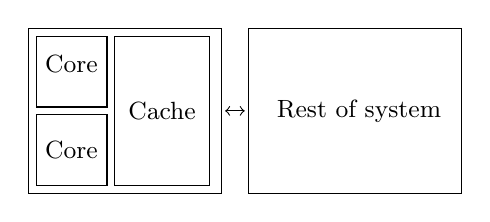
\begin{tikzpicture}
\draw (-0.5, -0.5) rectangle ++(0.9, 0.9);
\draw (-0.05, 0.05) node {\small Core};

\draw (-0.5, -1.5) rectangle ++(0.9, 0.9);
\draw (-0.05, -1.05) node {\small Core};

\draw (0.5, -1.5) rectangle ++(1.2, 1.9);
\draw (1.1, -.55) node {\small Cache};

\draw (-0.6, -1.6) rectangle ++(2.45, 2.1);

\draw (2.2, -1.6) rectangle ++(2.7, 2.1);
\draw (3.6, -0.55) node {\small Rest of system};

\draw[<->] (1.9, -0.55) -- (2.15, -0.55);
\end{tikzpicture}
\end{center}

  \begin{itemize}
    \item Each core can execute a different thread
    \item Shared memory quickly becomes the bottleneck
  \end{itemize}
\end{frame}

\begin{frame}
  \frametitle{Executing 2 Threads on a Single Core}

  \begin{center}
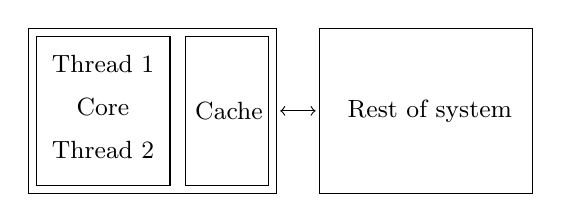
\begin{tikzpicture}
\draw (-1.4, -1.5) rectangle ++(1.7, 1.9);
\draw (-0.55, 0.05) node {\small Thread 1};
\draw (-0.55, -1.05) node {\small Thread 2};
\draw (-0.55, -0.5) node {\small Core};

\draw (0.5, -1.5) rectangle ++(1.05, 1.9);
\draw (1.05, -.55) node {\small Cache};

\draw (-1.5, -1.6) rectangle ++(3.15, 2.1);

\draw (2.2, -1.6) rectangle ++(2.7, 2.1);
\draw (3.6, -0.55) node {\small Rest of system};

\draw[<->] (1.7, -0.55) -- (2.15, -0.55);
\end{tikzpicture}
  \end{center}


    On a single core, must context switch between threads:
      \begin{itemize}
        \item every $N$ cycles; or
        \item wait until cache miss, or another long event
      \end{itemize}
    Resources may be unused during execution. \vfill

    Why not take advantage of this?

\end{frame}

\begin{frame}
  \frametitle{Executing M Threads on a N Cores}
\begin{center}
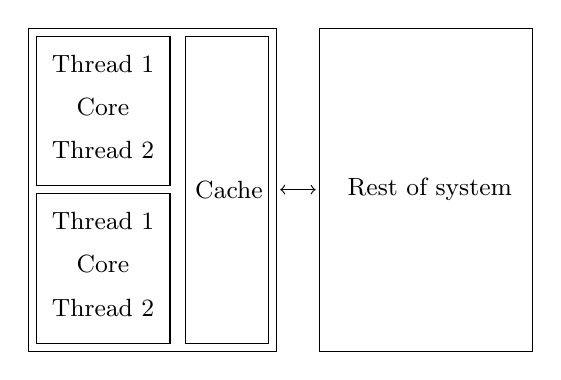
\begin{tikzpicture}

 \draw (-1.4, -1.5) rectangle +(1.7, 1.9);
 \draw (-1.4, -3.5) rectangle +(1.7, 1.9);

\foreach \y in {-2, 0}
{
 \draw (-0.55, 0.05) + (0, \y) node {\small Thread 1};
 \draw (-0.55, -1.05) + (0, \y) node {\small Thread 2};
 \draw (-0.55, -0.5) + (0, \y) node {\small Core};
}

\draw (0.5, -3.5) rectangle ++(1.05, 3.9);
\draw (1.05, -1.55) node {\small Cache};

\draw (-1.5, -3.6) rectangle ++(3.15, 4.1);

\draw (2.2, -3.6) rectangle ++(2.7, 4.1);
\draw (3.6, -1.55) node {\small Rest of system};

\draw[<->] (1.7, -1.55) -- (2.15, -1.55);
\end{tikzpicture}
\end{center}

\begin{changemargin}{2.5cm}
Here's a Chip Multithreading example. \vfill

UltraSPARC T2 has 8 cores, each of which supports 8 
threads. All of the cores share a common level 2 cache.
\end{changemargin}

\end{frame}

\begin{frame}
  \frametitle{SMT (Simultaneous Multithreading)}


    Use idle CPU resources (may be calculating or waiting
          for memory) to execute another task.
    \vfill
    Cannot improve performance if shared resources are the bottleneck.
    \vfill
    Issue instructions for each thread per cycle.
    \vfill
    To the OS, it looks a lot like SMP, but gives only up to 30\% performance improvement.
    \vfill
Intel implementation: Hyper-Threading.

\end{frame}

\begin{frame}
  \frametitle{Example: Non-SMP system}

\begin{center}
  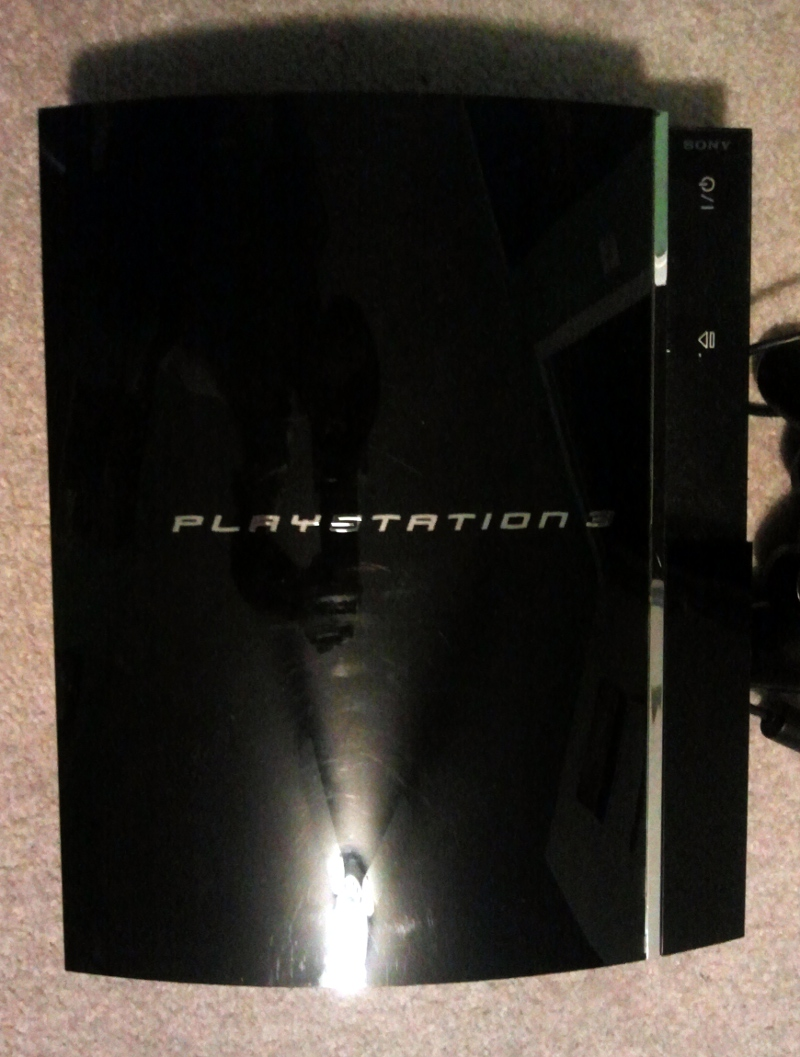
\includegraphics[height=.5\textheight]{images/ps3-small}
\end{center}

  PlayStation 3 contains a Cell processor:
  \begin{itemize}
    \item PowerPC main core (Power Processing Element, or ``PPE'')
    \item 7 Synergistic Processing Elements (``SPE''s): small vector computers.
  \end{itemize}
\end{frame}

\begin{frame}
  \frametitle{NUMA (Non-Uniform Memory Access)}


    In SMP, all CPUs have uniform (the same) access time for resources.
    \vfill
    For NUMA, CPUs can access different resources faster (resources: not just
          memory).
    \vfill
    Schedule tasks on CPUs which access resources faster.
    \vfill
    Since memory is commonly the bottleneck, each CPU has its own memory
          bank.

\end{frame}

\begin{frame}
  \frametitle{Processor Affinity}

\begin{center}
	
\includegraphics[width=0.4\textwidth]{images/traeger.jpg}
\end{center}

    Each task (process/thread) can be associated with a set of processors.
    \vfill
    Useful to take advantage of existing caches (either from the last time
          the task ran or task uses the same data).
    \vfill
    Hyper-Threading is an example of complete affinity for both threads on
          the same core.
    \vfill
    Often better to use a different processor if current set busy.

\end{frame}



\begin{frame}
\frametitle{Predict and Mispredict}
The compiler (\& CPU) take a look at code that results in branch instructions.

Examples: loops, conditionals, or the dreaded \texttt{goto}.

It will take an assessment of what it thinks is likely to happen. 

\end{frame}



\begin{frame}
\frametitle{Let's Not Predict}

In the beginning the CPUs/compilers didn't really think about this sort of thing.

They come across instructions one at a time and do them and that was that. 

If one of them required a branch, it was no real issue. 

Then we had pipelining...
\end{frame}



\begin{frame}
\frametitle{Not Just for Oil}

The CPU would fetch the next instruction while decoding the previous one, and while executing the instruction before. 

That means if evaluation of an instruction results in a branch, we might go somewhere else and therefore throw away the contents of the pipeline. 

Thus we'd have wasted some time and effort. 

If the pipeline is short, this is not very expensive.\\
\quad But pipelines keep getting longer... 

\end{frame}



\begin{frame}
\frametitle{Take a Guess}

The compiler and CPU look at instructions on their way to be executed and analyze whether it thinks it's likely the branch is taken. 

This can be based on several things, including the recent execution history. 

If we guess correctly, this is great, because it minimizes the cost of the branch. 

If we guess wrong, we flush the pipeline and take the performance penalty.

\end{frame}



\begin{frame}
\frametitle{Take a Hint}

The compiler and CPU's branch prediction routines are pretty smart.\\
\quad Trying to outsmart them isn't necessarily a good idea. 

But we can give the compiler (\texttt{gcc} at least) some hints about what we think is likely to happen. 

Our tool for this is the \texttt{\_\_builtin\_expect()} function, which takes two arguments, the value to be tested and the expected result.

\end{frame}


%%%%%%%%%%%%%%%%%%%%%%%%%%%%%%%%%%%%%%%%%%%%%%%%%%%%%%%%%%%%%%%%%%%%%%%%%%%%%%%%
\begin{frame}[fragile]
  \frametitle{Branch Prediction Hints}

\begin{center}
	
\includegraphics[width=0.4\textwidth]{images/hint.jpeg}
\end{center}
  
  {\tt gcc} allows you to give branch
  prediction hints by calling this builtin function:

  \begin{center}
    \verb+long __builtin_expect (long exp, long c)+
  \end{center}

  The expected result is that {\tt exp} equals {\tt c}.\\[1em]
  Compiler reorders code \& tells CPU the prediction.
  
  
\end{frame}
%%%%%%%%%%%%%%%%%%%%%%%%%%%%%%%%%%%%%%%%%%%%%%%%%%%%%%%%%%%%%%%%%%%%%%%%%%%%%%%%



\begin{frame}[fragile]
\frametitle{Check the Header}

In the linux \texttt{compiler.h} header there are two neat little shortcuts defined:

\begin{verbatim}
# define likely(x)      __builtin_expect(!!(x), 1)
# define unlikely(x)    __builtin_expect(!!(x), 0)
\end{verbatim}

Compile with at least optimization level 2 (\texttt{-O2}) to get the compiler to take these hints at all.

\end{frame}



\begin{frame}[fragile]
\frametitle{Force a Mispredict}
{\scriptsize
\begin{verbatim}
        #include <stdlib.h>
        #include <stdio.h>

        static __attribute__ ((noinline)) int f(int a) { return a; }

        #define BSIZE 1000000
        int main(int argc, char* argv[]) 
        {
          int *p = calloc(BSIZE, sizeof(int));
          int j, k, m1 = 0, m2 = 0;
          for (j = 0; j < 1000; j++) {
            for (k = 0; k < BSIZE; k++) {
              if (__builtin_expect(p[k], EXPECT_RESULT)) {
                m1 = f(++m1);
              } else {
                m2 = f(++m2);
              }
            }
          }

          printf("%d, %d\n", m1, m2);
        }
\end{verbatim}
}

\end{frame}



\begin{frame}[fragile]
\frametitle{Mispredict Results}

Running it yielded:
{\scriptsize
\begin{verbatim}
plam@plym:~/459$ gcc -O2 likely-simplified.c -DEXPECT_RESULT=0 -o likely-simplified
plam@plym:~/459$ time ./likely-simplified
0, 1000000000

real	0m2.521s
user	0m2.496s
sys	0m0.000s
plam@plym:~/459$ gcc -O2 likely-simplified.c -DEXPECT_RESULT=1 -o likely-simplified
plam@plym:~/459$ time ./likely-simplified
0, 1000000000

real	0m3.938s
user	0m3.868ss
sys	0m0.000s
\end{verbatim}
}
\end{frame}



\begin{frame}
\frametitle{Hint Results}

In the original source the author reports the following results.

Scanning a one million element array, with all elements initially zero, the results are:

\begin{itemize}
	\item No use of hints: \texttt{0:02.68 real,  2.67 user, 0.00 sys}
	\item Good prediction: \texttt{0:02.28 real,  2.28 user, 0.00 sys}
	\item Bad prediction: \texttt{0:04.19 real,  4.18 user, 0.00 sys}
\end{itemize}

When about one in ten thousand values in the array is nonzero, then it's roughly the ``break-even'' point for the setup as described.

Conclusion: it's hard to outsmart the compiler. Maybe it's better not to try.

\end{frame}



\begin{frame}
\frametitle{More About Branch Prediction}

I want you to pick up two points from this discussion:

\begin{itemize}
\item How branch predictors work
\item Applying a (straightforward) expected value computation to predict performance.
\end{itemize}



\end{frame}


\begin{frame}[fragile]
\frametitle{Branch Prediction \& Misprediction}

\begin{minipage}{.4\textwidth}
\begin{center}
	
\includegraphics[width= \textwidth]{images/Two-Buttons.jpg}
\end{center}
\end{minipage}
\hspace*{2em} \begin{minipage}{.4\textwidth} \begin{lstlisting}
branch_if_not_equal x, 0, else_label
// Do stuff
goto end_label
else_label:
// Do things
end_label:
// whatever happens later
\end{lstlisting}
\end{minipage}

\end{frame}



\begin{frame}
\frametitle{No Prediction}

With no prediction, we need to serialize:

\begin{center}
\begin{tabular}{c|c|c|c}
bne.1 & bne.2 \\ \hline
& & things.1 & things.2
\end{tabular}
\end{center}

\end{frame}



\begin{frame}
\frametitle{Predict Things}
If our prediction is correct, we save time.

\begin{center}
\begin{tabular}{c|c|c}
bne.1 & bne.2 \\ \hline
& things.1 & things.2 \\
\\
\end{tabular}
\end{center}

But we might be wrong and need to throw out the bad prediction.

\begin{center}
\begin{tabular}{c|c|c|c}
bne.1 & bne.2 \\ \cline{1-2}
& \sout{things.1} \\ \hline
& & stuff.1 & stuff.2
\end{tabular}
\end{center}


\end{frame}



\begin{frame}
\frametitle{Cartoon Model}

We need to quantify the performance.


Let's pretend that our pipelined
CPU executes, on average, one instruction per clock.

Mispredicted branches cost 20 cycles, while correctly-predicted
branches cost 1 cycle. 

We'll also assume that the instruction
mix contains 80\% non-branches and 20\% branches. 

So we can predict
average cycles per instruction.


\end{frame}

\begin{frame}
\frametitle{Prediction Quantification}

\begin{center}
	
\includegraphics[width=0.5\textwidth]{images/math.jpg}
\end{center}

With no prediction (or always-wrong prediction):
\[
\mathrm{non\_branch\_\%} \times 1 \mathrm{~cycle} + \mathrm{branch\_\%} \times 20 \mathrm{~cycles} = 4.8 \mathrm{~cycles}.
\]
With perfect branch prediction:
\[
\mathrm{non\_branch\_\%} \times 1 \mathrm{~cycle} + \mathrm{branch\_\%} \times 1 \mathrm{~cycle} = 1 \mathrm{~cycle}.
\]
So we can make our code run 4.8$\times$ faster with branch prediction!

\end{frame}


\begin{frame}
\frametitle{Strategy 1: Predict Taken}

We can predict that a branch is always taken. 

If we got 70\% accuracy, then our cycles per instruction would be:
\[
(0.8 + 0.7 \times 0.2) \times 1 \mathrm{~cycle} + (0.3 \times 0.2) \times 20 \mathrm{~cycles} = 2.14 \mathrm{~cycles}.
\]
The simplest possible thing already greatly improves the CPU's average throughput.

\end{frame}



\begin{frame}
\frametitle{BTFNT - Dynamite}

Let's leverage that observation about loop branches to do better.
Loop branches are, by definition, backwards. 

So we can design a branch predictor which predicts ``taken''
for backwards and ``not taken'' for forwards. 

Let's say that this might get us to 80\% accuracy. 

\[
(0.8 + 0.8 \times 0.2) \times 1 \mathrm{~cycle} + (0.2 \times 0.2) \times 20 \mathrm{~cycles} = 1.76 \mathrm{~cycles}.
\]


The PPC 601 (1993) and 603 used this scheme.

\end{frame}


\begin{frame}
\frametitle{Dynamic}

So far, we will always make the same prediction at each branch---known as a
\alert{static} scheme. 

But we can do better by using what recently happened to
improve our predictions. 

This is particularly important when program execution
contains distinct phases, with distinct behaviours.


We therefore move to \alert{dynamic} schemes.

\end{frame}



\begin{frame}
\frametitle{Remember Your History}

For every branch,
we record whether it was taken or not last time it executed (a 1-bit scheme).


Of course, we can't store all branches. 

So let's use the low 6 bits of the address
to identify branches. 

Doing so raises the prospect of \emph{aliasing}:
different branches (with different behaviour) map to the same spot in the table.

We might get 85\% accuracy with such a scheme.
\[
(0.8 + 0.85 \times 0.2) \times 1 \mathrm{~cycle} + (0.15 \times 0.2) \times 20 \mathrm{~cycles} = 1.57 \mathrm{~cycles}.
\]

At the cost of more hardware, we get noticeable performance improvements. The DEC EV4 (1992) and
MIPS R8000 (1994) used this one-bit scheme.

\end{frame}


\begin{frame}
\frametitle{Two-Bit Scheme}

What if a branch is almost always taken but occasionally not taken (e.g. TTTTTTNTTTT)?

We get penalized twice
for that misprediction: once when we mispredict the not taken, and once when we mispredict the next taken. 

So, let's store whether a branch is ``usually'' taken, using a so-called
2-bit saturating counter.

Every time we see a taken branch, we increment the counter for that
branch; every time we see a not-taken branch, we decrement. 

\end{frame}


\begin{frame}
\frametitle{Two-Bit Scheme}

If the counter is 00 or 01, we predict ``not taken''; if it is 10 or
11, we predict ``taken''.

With a two-bit counter, we can have fewer entries at the same size, but they'll do better.
It would be reasonable to expect 90\% accuracy.
\[
(0.8 + 0.9 \times 0.2) \times 1 \mathrm{~cycle} + (0.1 \times 0.2) \times 20 \mathrm{~cycles} = 1.38 \mathrm{~cycles}.
\]

This was used in a number of chips, from the LLNL S-1 (1977) through the Intel Pentium (1993).



\end{frame}


\begin{frame}[fragile]
\frametitle{Two-Bit Adaptive, Global}

We're still not taking patterns into account. Consider the following {\tt for} loop.
\begin{lstlisting}[language=C]
for (int i = 0; i < 3; ++i) {
  // code
}
\end{lstlisting}
The last three executions of the branch determine the next direction:
\begin{verbatim}
 TTT => N
 TTN => T
 TNT => T
 NTT => T
\end{verbatim}

Let's store what happened the last few times we were at a particular address---the
\alert{branch history}. 

\end{frame}



\begin{frame}
\frametitle{Two-Bit Adaptive, Global}

From a branch address and history, we derive an index, which
points to a table of 2-bit saturating counters. 

What's changed from the two-bit scheme
is that the history helps determine the index and hence the prediction.

This scheme might give something like 93\% accuracy.
\[
(0.8 + 0.93 \times 0.2) \times 1 \mathrm{~cycle} + (0.07 \times 0.2) \times 20 \mathrm{~cycles} = 1.27 \mathrm{~cycles}.
\]

The Pentium MMX (1996) used a 4-bit global branch history.

\end{frame}



\begin{frame}
\frametitle{Two-Level Adaptive, Local}


The change here is that the CPU keeps a separate history for each branch.


So the branch address determines which branch history gets used.


We concatenate the address and history to get the index, which then points to a
2-bit counter again. 

We are starting to encounter diminishing returns, but we might
get 94\% accuracy:
\[
(0.8 + 0.94 \times 0.2) \times 1 \mathrm{~cycle} + (0.06 \times 0.2) \times 20 \mathrm{~cycles} = 1.23 \mathrm{~cycles}.
\]

The Pentium Pro (1996), Pentium II (1997) and Pentium III (1999) use this.


\end{frame}



\begin{frame}
\frametitle{gshare}

Instead of concatenating the address and history, we can xor them. 

This allows
us to use more bits for both the history and address. 

This keeps the accuracy the same,
but simplifies the design.


\end{frame}



\begin{frame}
\frametitle{Other Predictors}

 We can build (and people have built) more sophisticated predictors.


These predictors could, for instance, better handle aliasing, where
different branches/histories map to the same index in the table.

\end{frame}


\begin{frame}
\frametitle{Hacking Time... Hacking Too Much Time}

\begin{center}
	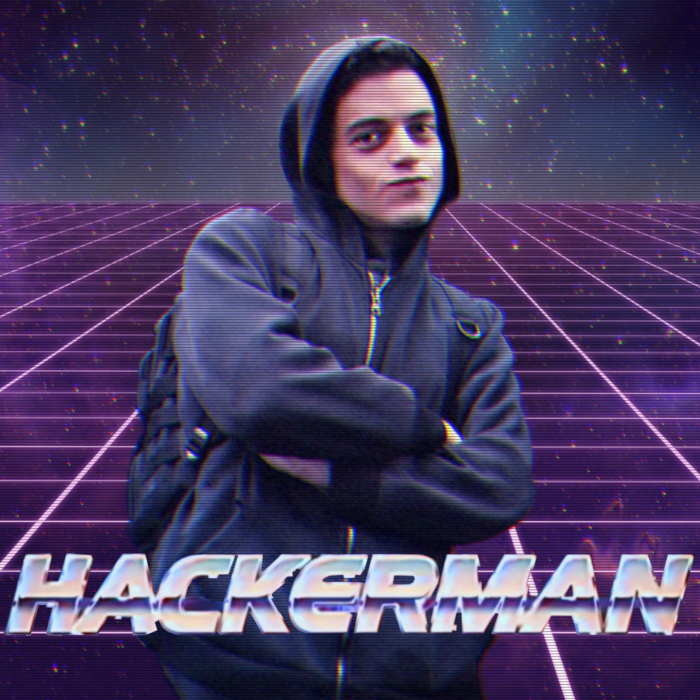
\includegraphics[width=0.6\textwidth]{images/hackerman.png}
\end{center}

\end{frame}


\begin{frame}
\frametitle{We Are Under Attack!}

There's been a lot happening lately in terms of exploiting the hardware of CPU architectures to get access to privileged data. 

Unfortunately these things have performance implications!

\end{frame}


\begin{frame}
\frametitle{Cache side-channel attacks}

\begin{center}
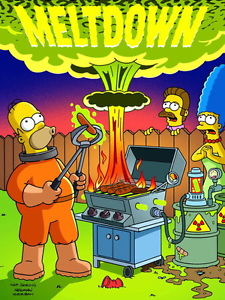
\includegraphics[width=0.25\textwidth]{images/meltdown.jpg}
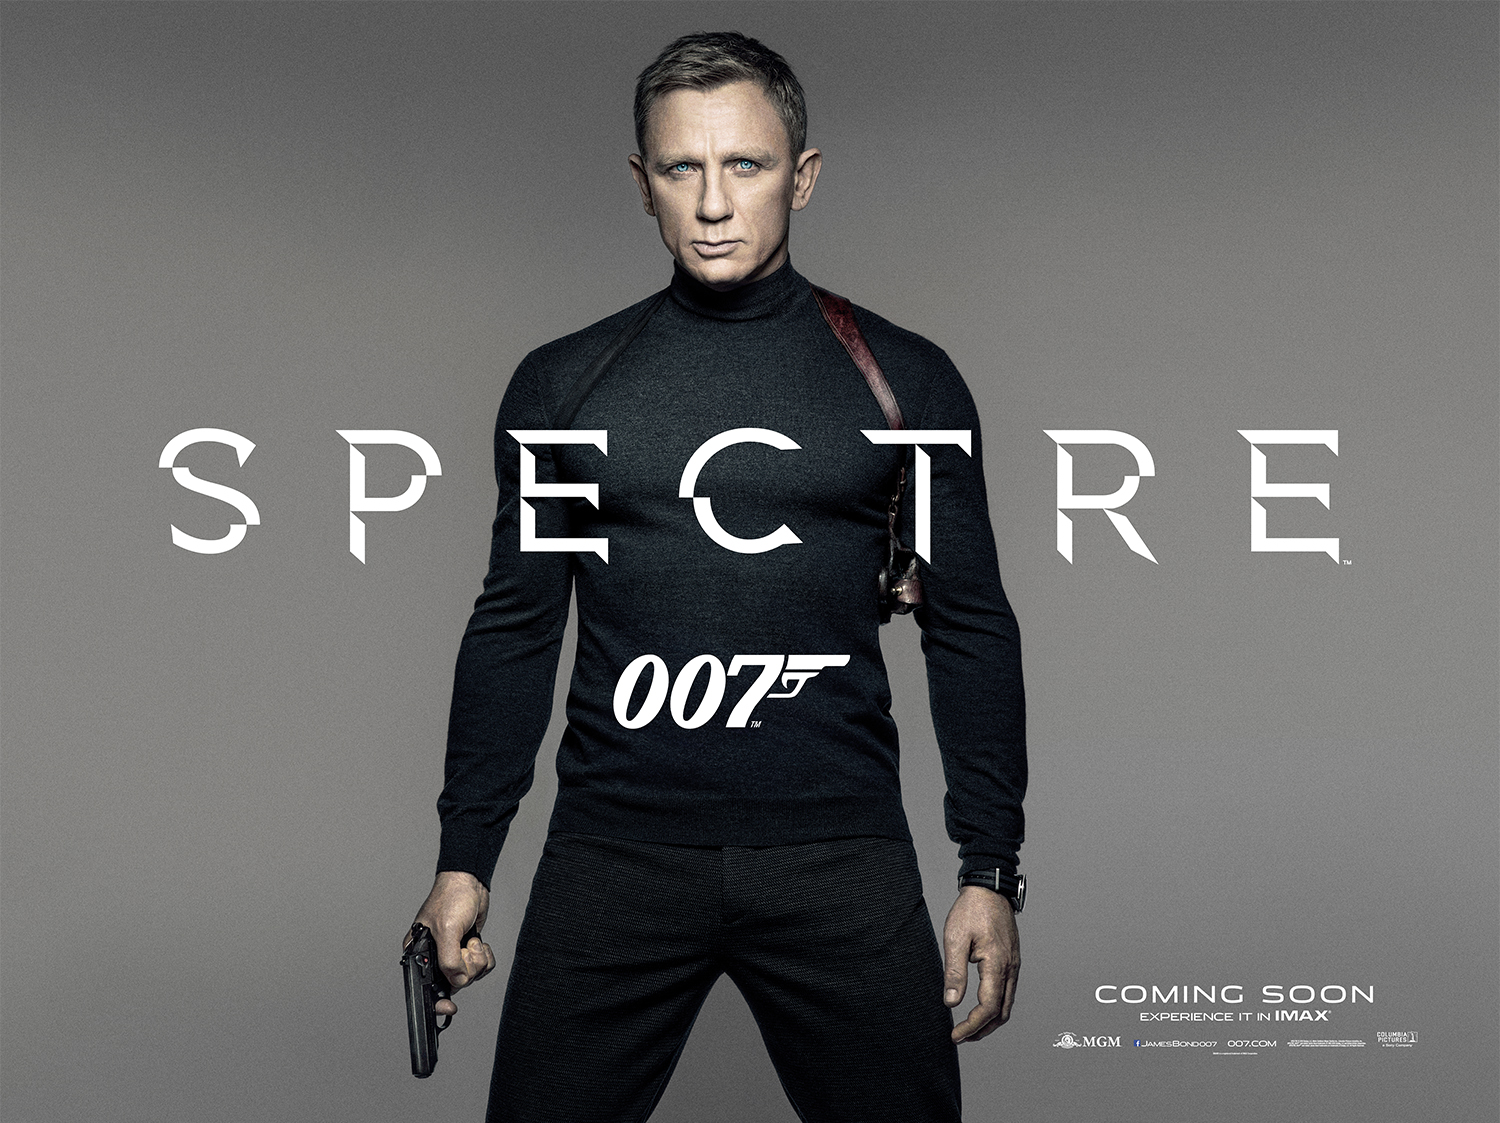
\includegraphics[width=0.40\textwidth]{images/spectre.jpg}
\end{center}

\end{frame}



\begin{frame}
\frametitle{Cache side-channel attacks}

\begin{center}

\includegraphics[width=0.8\textwidth]{images/meltdown-spectre.png}
\end{center}


\end{frame}

\begin{frame}
\frametitle{Cache Side-Channel Attacks}

These attacks leverage performance features of modern CPUs to break process isolation guarantees.

In principle, a process shouldn't be able to read memory that belongs to the kernel or to other processes.

Spectre and Meltdown can cause privileged memory to be loaded into the cache, and then extracted using a cache side-channel attack.

Mitigation: more isolation, lower performance.

\end{frame}



\begin{frame}
\frametitle{Vulnerability Example}

\begin{center}
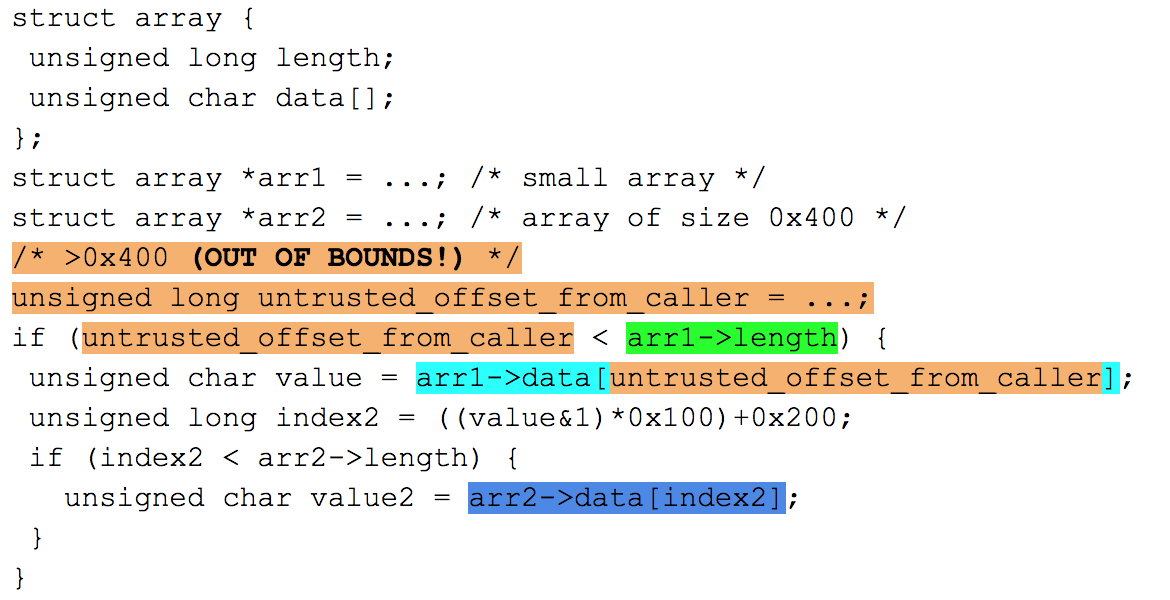
\includegraphics[width=0.8\textwidth]{images/cache-sidechannel1.png}
\end{center}
\tiny (from \url{https://hk.saowen.com/a/81873c7b149c0993836e8a4fa4f879b4178085a3ad14c09a5f22f5a9c76373ca})

\end{frame}

\begin{frame}
\frametitle{Hyperthreading Attacks}
Remember that in hyperthreading, two threads are sharing the same execution core. That means they have hardware in common. 

Because of this, a thread can figure out what the other thread is doing!

By noticing its cache accesses and by timing how long it takes to complete operations.

Attack name: PortSmash

\end{frame}

\begin{frame}
\frametitle{Hyperthreading Attacks}
In the practical example, a 384-bit secret key is (over time) completely stolen by another process. 

Mitigation: prevent threads from different processes from using the same core... 

Possibly the only long term solution is to not use hyperthreading at all... 

The performance implications of which are obvious \& significant!


\end{frame}

\end{document}
